% https://github.com/martinhelso/phduio-monograph

% Add [final] to remove marginal notes,
% remove [colophon] for a blank colophon page:
\documentclass[final, nocolophon, english, oneside, screen]{phduio}

\usepackage{phdstyle}   % Custom style

\usepackage{wrapfig}

\usepackage{longtable}

\usepackage{arydshln}

\let\printglossary\relax
\let\theglossary\relax
\let\endtheglossary\relax
\usepackage[acronym, toc, nohypertypes={acronym}]{glossaries}
\makeglossaries
\newacronym[plural=ADAS,firstplural=Advanced driver assistance systems (ADAS)]{adas}{ADAS}{Advanced driver assistance system}

\newacronym[plural=POMDP,firstplural=Partially observable Markov decision processes (POMDP)]{pomdp}{POMDP}{Partially observable Markov decision process}

\newacronym{rl}{RL}{reinforcement learning}

\newacronym{irl}{IRL}{inverse reinforcement learning}

\newacronym{torcs}{TORCS}{The Open Racing Car Simulator}

\newacronym{hitl}{HITL}{Human-in-the-loop}

\newacronym{mpc}{MPC}{Model Predictive Control}

\newacronym[plural=MDP,firstplural=Markov decision processes (MDP)]{mdp}{MDP}{Markov decision process}

\newacronym{lkas}{LKAS}{Lane Keep Assist System}

\newacronym{act-r}{ACT-R}{Adaptive Control of Thought-Rational}

\newacronym[plural=POMCP,firstplural=Partially observable Monte-Carlo Planning (POMCP)]{pomcp}{POMCP}{Partially observable Monte-Carlo Planning}

\newacronym{pbvi}{PBVI}{Point-based Value Iteration}

\newacronym{hsvi}{HSVI}{Heuristic Search Value Iteration}

\newacronym{ucb1}{UCB1}{Upper Confidence Bounds 1}

\newacronym{despot}{DESPOT}{Determinized sparse partially observable tree}

\newacronym{mcts}{MCTS}{Monte Carlo tree search}

\newacronym{labecop}{LABECOP}{Lazy Belief Extraction for Continuous Observation POMDPs}


\author{Jokke Mats Jansen}
\title{Master's Thesis proposal}
%\subtitle{Optional Subtitle}
\department{Artificial Intelligence}
\faculty{Faculty of Science}
\affiliation
{
    \textbf{Supervisors}
    \and
    \makebox[.16\linewidth][l]{First:} Dr. Shihan Wang
    \and
    \makebox[.16\linewidth][l]{Second:} Dr. Leendert van Maanen
}


\includeonly
{
    % sections/dedication,
    % sections/abstract,
    % sections/preface,
    sections/introduction,
    sections/problem,
    sections/algorithm,
    sections/pomcp,
    sections/literature,
    sections/experiment,
    sections/plan,
}

\begin{document}

    \frontmatter        % Folios in Roman numerals, unnumbered chapters.

    \uiotitle

    % \include{sections/dedication}
    % \chapter{Abstract}
\label{sec:abstrac}

Driver assistance systems are paving the way for automated driving. Until fully autonomous driving will be available and in wide-spread use, assistance systems, such as lane-keeping assistance, can help prevent accidents by supporting a human driver. However, if a lane-keeping assistance system strongly restricts the driver's autonomy, the driver may overly trust the system \parencite{over-trust} and distract herself more frequently \parencite{driver-distraction}. It is advantageous to base the intensity of assistance on the attentiveness of the driver (see \cite{disracted-lane-keeping-1} and \cite{disracted-lane-keeping-2}). Thereby, the driver is kept in the loop when attentive but is supported during periods of distraction. Driver distraction is a serious issue; 14\% of crashes in the USA were affected by distracted driving in 2018 \parencite{distracted_nhtsa}. Taking into account the driver's distraction for the activation of assistance technology could help prevent such accidents.

We design an agent as a lane-keeping assistant that shares control of the vehicle with the driver. The driver's distraction is estimated online, allowing the agent to assist a distracted driver while keeping an attentive driver in control. For the estimation of the driver's distraction, the agent relies solely on driving performance measures, such as the driver's steering movements and sensory information about the vehicle's position. To account for uncertainty about the driver's distraction and the exact position of the vehicle, the problem is modeled as a \acrfull{pomdp}. To the best of our knowledge, this is the first study using only commonly available driving performance metrics instead of sophisticated driver monitoring systems to estimate the driver's distraction with a POMDP.

We apply the \acrfull{pomcp} algorithm \parencite{pomcp} to solve the POMDP online. The algorithm performs Monte-Carlo tree search, sampling possible future scenarios to form a strategy. Our experiments confirm that the driver's overall lane-keeping performance is significantly enhanced. Our approach has potential. However, there are obstacles that have to be overcome for the method to be viable in practice. First, the solver is not efficient enough; planning takes too much time. Second, we use simple hand-crafted driver models for our experiments. The driver model can and should be replaced by a more sophisticated and realistic model. Third, our method relies on the discretization of the action and observation spaces. A car's sensory information and steering actions are naturally continuous. We discuss these limitations in detail and provide suggestions for future improvements.


% \begin{enumerate}
%     \item How can a lane-keeping scenario with shared control between a potentially distracted human driver and an agent be modeled using a POMDP?
%     \item Can the agent estimate the driver's distraction using driver performance measures alone, allowing it to take appropriate actions when the driver becomes distracted?
%     \item Is the solution approach viable for a real-world scenario, and if not, what limitations are there, and what are potential methods to solve them?
% \end{enumerate}

% \begin{enumerate}
%     \item We provide a POMDP model with a continuous state as a representation of the shared control lane-keeping scenario, outlining how both the human driver and the car's dynamic can be simulated. 
%     \item Our model for the human driver is simple. However, our modeling approach is also suitable for the integration of a more sophisticated driver model (see section \ref{sec:complex-driver}).
%     \item We enable an agent to act as a lane-keeping assistant to the driver, taking into account the driver's potential distraction. The POMDP is solved online by applying the POMCP algorithm. Experimental results show that the driving performance is enhanced.
%     \item Particle deprivation is a common problem with a particle filter approach such as POMCP. Implementing particle injection (see section \ref{sec:particle_deprivation}) and introducing domain knowledge by the use of preferred actions (see section \ref{sec:preferred_actions}) leads to an improvement.
%     \item Using the TORCS driving simulator as a generative model during planning with POMCP is not efficient enough for a real-time scenario. The performance needs to be significantly optimized. Suggestions on how to achieve this are provided in section \ref{sec:perf_opt}.
%     \item The lane-keeping performance of our approach is inferior to traditional lane-keeping assistance systems. The immediate application of the approach is not advisable. Section \ref{sec:future} outlines opportunities for improvement.
%     \item Our simulation method allows for a repetition of experiments. Problems can be revisited and analyzed. This is important in the safety-critical domain of automated driving.
% \end{enumerate}
    % \include{sections/preface}

    % \cleartorecto
    \microtypesetup{protrusion = false}
    \tableofcontents*    % Or \tableofcontents*
    % \cleartorecto
    % \listoffigures      % Or \listoffigures*
    % \cleartorecto
    % \listoftables       % Or \listoftables*
    \microtypesetup{protrusion = true}
    
    \clearpage
    \printglossary[type=\acronymtype]
    
    \mainmatter         % Folios in Arabic numerals, numbered chapters.

    \chapter{Introduction}
\label{sec:intro}

\iffalse

Driver   inattention: inattention  occurs  when  the  driver’s  allocation  of resources  to  activities  does not  match  the  demands  of  activities  required  for  the control of safety margins.

Driver distraction: where  the  driver  allocates  resources  to a  non-safety critical activity while the resources allocated to activities critical for safe driving do not match the demands of these activities.

Types of distraction:
    Visual: taking your eyes off the road
    Manual: taking your hands off the wheel
    Cognitive: taking your mind off driving2                             

DISTRACTION

Visual distraction or cognitive distraction have been investigated by combining vehicle state [36], [147], [148], drivers’ visual state [145]–[147], [149], and operations [147], [149], [191]. Answers to the question of how to measure a driver’s cognitive distraction have been given in [150]. Learning-based approaches such as deep sparse autoencoders [192], deep belief networks or DBNs [188], support vector machines (SVM) [145], [193] have been widely used to detect and classify driver distraction. \cite{shared_control}


COGNITIVE MODEL

One of the most utilized means is based on the “adaptive control of thought-rational (ACT-R) [141]”
cognitive where the discrete nature of drivers’ control actions is captured from a cognitive perspective. For example, Salvucci et al. developed an integrated cognitive pathfollowing driver model [142] and lane-change driver model [143] using the combination of the ACT-R cognitive architecture and perceptual-motor process. \cite{shared_control}



It is well known that manual control is prone to human errors. On the other hand, fully automated tasks are currently subject to wide-ranging limitations in decision-making and situationawareness. To exploit full potentials of both of human and automation while overcoming the barriers of car-to-driver transition, Mulder et al. [27] presented an entirely different control scheme – shared control systems3. The human driver and the automated driving agent continuously share and cooperatively complete a specific driving task, thereby allowing drivers to enjoy driving while keeping in control consistently. Moreover, the shared-control scheme can synergize innate human capacities and technological capabilities to enable us to realize our full potential [31].



Keeping the lane is one of the primary tasks of controlling a vehicle. Especially on longtrips  on  extra-urban  roads  this  might  be  a  monotonous  and  annoying  taskwhere unintended lane departures may occur caused  by momentary lapses  ofattention or drowsiness. As a consequence of an unintended lane departure theremight happen a
●Collision with a stationary object
●Collision with a vehicle traveling in the same direction
●Collision with oncoming traffic●Rollover accident
●Collision with pedestrians and bicyclists beside the road
●Further accident caused by failed corrective steering and braking (loss of vehiclecontrol)

Generally speaking unintended lane departures are one major cause of severeaccidents. However, there might be various root causes of an unintended lane depar-ture like driver distraction, drowsiness, a temporary blackout of the driver, toohigh velocity (especially in curves), poor visibility of lane markers and road geometry,and more. These chains of cause and effect need to be considered for defining thescope  of  lane  keeping  and  lane  departure  warning  systems  as  well  as  theireffectiveness

https://link.springer.com/referenceworkentry/10.1007%2F978-0-85729-085-4_26

Theconcept of Honda LKA systems is based on a cooperative operation between driver andvehicle intended to lighten the operation load but at the same time not to diminish drivermotivation (Ishida et al.2003).


the road to hell is paved with good intentions…
https://delfthapticslab.nl/project/responsible-adaptation-of-lane-keeping-assistance/

How can we assist drivers in lane-keeping, without inducing them to misuse this assistance to drive faster? This question relates to behavioral adaptation: a central concept in the design of assistance systems that we know in daily life as “the road to hell is paved with good intentions…”. It states that when we design systems that support humans, they often adapt their behavior in a way that mitigates the very benefits that the system aimed to realize. Advanced driver assistance systems (ADAS) are a well-known example of designs were anticipated safety benefits are diminished because drivers show undesired behavioral adaptations. Literature shows that ADAS lead to increased risk-taking, such as driving at a higher speed, driving closer to a lead vehicle, or performing distractive non-driving tasks[1].

\fi

%
% Overview first: Tell a story
%

\section{Motivation}

Fully autonomously driving cars have the potential to rule out human driving error which is at least a contributing factor to most accidents today. Many social and technical obstacles have yet to be overcome until fully autonomous cars become market-ready \parencite{autonomous_driving_book}. However, many \glspl{adas} such as adaptive cruise control, lane keeping and changing assistance, and automated collision mitigation are already deployed in modern cars. 

The extend to which an \gls{adas} takes control varies. While the potential prevention of human-error caused accidents increases with the elaborateness of intervention by an assistant system, excessive intervention drastically limits the driver's autonomy. A loss of driver autonomy can turn driving into a monotonous and tedious supervisory task. Drivers easily become inattentive and are more prone to distract themselves, for example by looking on their phone. However, as long as assistance systems are not sufficient to handle all situations, a concentrated human will remain necessary to take actions in situations the assistance system fails. Leaving the driver with a pure supervision task can lead to a long transition time for the driver when it is required to retake control of the vehicle \parencite{shared_control}. Being in control means having to concentrate. Therefore, the goal should be to keep the human driver in control as much as possible but to assist when help is really needed. As a result, driving pleasure is enhanced and drivers are prevented from relying too heavily on the assistance systems.

% Human drivers and \gls{adas} often already \emph{share} the control over the car.

% The extend to which an \gls{adas} takes control varies. Some systems only suggest actions to the driver, others actively intervene in steering, acceleration, or braking, and semi-automated systems assume full authority over the car's control, leaving the driver only with the task of supervision. While the potential prevention of human-error caused accidents increases with the elaborateness of intervention by an \gls{adas}, excessive intervention drastically limits the driver's autonomy. 

% Leaving the driver with a pure supervision task can lead to over-trust, neglect and complacency and may result in a long transition time for the driver when it is required to retake control of the vehicle \parencite{shared_control}. 

% Shared control of the car by a human driver and an agent acting as \gls{adas} allows to exploit both the human's and the agent's unique qualities. 

% TODO: Add source for claim of different behavior when inattentive?
15\% of injury crashes in the US were associated with driver distraction in 2018 \parencite{distracted_nhtsa}. Therefore, it seems reasonable to make the extend of the \gls{adas}'s activation dependent on the driver's level of attention. Whenever a driver is inattentive or distracted, an \gls{adas} needs to be particularly sensitive. Yet in what way can an assistance system detect that a driver is distracted? 

\section{Problem overview}


% TODO: Add literature to back up eye tracking machine learing claim
There have bee attempts to develop systems that determining the psychological state of a driver in real time while driving. The application of eye tracking technology or analysis of camera footage using machine learning models is conceivable and has led to promising results. However, as promising as promising as these methods are, they are not readily available yet. Furthermore, they are quite intrusive and could be seen as an encroachment on privacy. Thus, the driver's level of attention is essentially unknown. Nevertheless, one can assume that distracted drivers act differently. Among other things, deviations such as increased reaction times and altered steering behavior are likely.

% If any of clues are noticeable, the system needs to lower its activation threshold.

% Besides  the  per-ception,  autonomous  driving  systems  constitute  of  multipletasks where classical supervised learning methods are no moreapplicable.  First,  when  the  prediction  of  the  agent’s  actionchanges  future  sensor  observations  received  from  the  envi-ronment under which the autonomous driving agent operates,for  example  the  task  of  optimal  driving  speed  in  an  urbanarea.  Second,  supervisory  signals  such  as  time  to  collision(TTC),  lateral  error  w.r.t  to  optimal  trajectory  of  the  agent,represent  the  dynamics  of  the  agent,  as  well  uncertainty  inthe  environment.  Such  problems  would  require  defining  thestochastic cost  function to be  maximized. Third, the  agent isrequired  to  learn  new  configurations  of  the  environment,  aswell  as  to  predict  an  optimal  decision  at  each  instant  whiledriving in its environment. This represents a high dimensionalspace given the number of unique configurations under whichthe agent & environment are observed, this is combinatoriallylarge. In all such scenarios we are aiming to solve a sequential decision  process,  which  is  formalized  under  the  classicalsettings  of  Reinforcement  Learning  (RL),  where  the  agent  isrequired  to  learn  and  represent  its  environment  as  well  asact  optimally  given  at  each  instan


A two-fold problem arises: On the one hand, a lane keeping assistance system has to be able to identify when drivers are distracted by observing their behavior. On the other hand, the system must have the capability to provide meaningful assistance. 



Intuitively, it seems reasonable to solve both problems individually; using a model that takes the available data, such as the driver's steering behavior, as input to classify whether the driver is distracted, and another model that assists a distracted driver in steering the car. Both could be trained using example data. However, this supervised approach entails two challenges: First, driving is a sequential decision process. An action influences future actions and driving situations in which decisions have to be made are essentially unique. Second, an activation of the assistance system can affect on how drivers behave. Drivers may adjust to the system. It is not possible to create a dataset that covers these dynamics entirely.


%to learn
%the differences in driving styles between attentive and distracted drivers from example data using supervised machine learning and then use this insight to conditionally intensify an \gls{adas} assistance. 



\Gls{rl} allows a system to learn and represent its behavior by interacting with it rather than learning from past experience. Therefore, \gls{rl} constitutes a promising method to develop an \gls{adas} or even a fully autonomous driving agent and its application in this area is a very active research area with many successful results \parencite{rl_driving_survey}. Because learning is achieved by exploration rather than from examples, \gls{rl} is able to perform well in sequential decision making tasks. Moreover, reinforcement learning algorithms can be extended to support learning with a partially observable state \parencite[p.~466]{RL_introductio}. While the agent can perceive the car's environment with sensors, the attention level of the driver is hidden. Nevertheless, only one \gls{rl} agent is needed to both learn how to assist in driving and to classify when this is desired due to a distracted driver.

The result is a shared control scenario where both the human driver and the agent can actively control (e.g. steer, brake, accelerate) the car simultaneously. Each can indirectly perceive the actions of the other by observing the state of the car. Thereby, on the one hand, the agent is able to analyze the driving behavior of the human and, on the other hand, the human can notice the assistance of the agent and may adapt to it. 

% TODO: interaction loop

% Offline: specify, prior to the execution, the best action to execute for all possible situations.

% While these approximate algorithms can achieve very good performance, they often take significant time (e.g. more than an hour) to solve large problems, where there are too many possible situations to enumerate (let alone plan for). Furthermore, small changes in the environment’s dynamics require recomputing the full policy, which may take hours or days.

% Whereas an offline search would compute an exponentially large contingency plan considering all possible happenings, an online search only considers the current situation and a small horizon of contingency plans.



Learning in a real-world situation is not feasible in the context of this thesis. Despite the inevitable high safety risk, it would also require an enormous investment of resources, and the complexity of a real-world driving scenario represents an insurmountable obstacle. Instead, the agent learns in a simulation environment with a simulated human driver. \gls{torcs}, a racing car simulator that allows to model various driving situations \parencite{torcs} is used as simulation environment. It offers a good balance between realism and resource efficiency and has been utilized in many papers regarding \gls{rl}-based driving before. An \gls{act-r} cognitive model is employed to simulate the human's actions. The model is able to keep the car in its lane, perform lane changes, and avoid collision with other road users. It captures behavioral differences between attentive and inattentive human drivers. Furthermore, a human-subject experiment is performed in the \gls{torcs} simulation environment to identify if the agent is able to generalize well enough to be useful for actual human drivers.

\section{Related work and contributions}

% See (POMDP, POMCP, Thesis) Towards Human-Like Prediction and Decision-Makingfor Automated Vehicles in Highway Scenarios

The main goal and differentiator of this thesis is to utilize reinforcement learning for a shared-control driving task with unknown attention of the human driver. One of the main challenges is that near real-time decisions of the agent are necessary. This drastically limits the time available for online planning. Accordingly, the implementation needs to be very efficient. Solving the problem using an algorithm that requires discretized states (e.g. steering angle categories) is contrasted with a solution using an algorithm directly supporting continuous states.


\section{Outline}

The rest of the proposal is organised as follows:
\begin{description}
    \item[\cref{sec:problem}]
    describes the problem in a formal manner using a \gls{pomdp}.
    
    \item[\cref{sec:literature}]
    summarizes and reviews important literature that serves as the foundation of the thesis.
    
    \item[\cref{sec:plan}]
    presents the initial research plan for the rest of the thesis, including important milestones and deadlines.
\end{description}


\iffalse

\cite{hitl_pomdp} define a similar \gls{pomdp} problem. An agent is supposed to activate a warning signal if the driver is drowsy and actively interfere by steering the car if the warning is unsuccessful in alerting the driver. The model representing the transition probabilities of the driver's interal state and action choice in \cite{hitl_pomdp} are arbitrarily constructed and likewise very simplified. A more realistic driving setting also requires a more sophisticated driver model. 


% An offline randomized point-based value iteration approach is employed to solve the POMDP for an approximate optimal policy. The policy is computed by iteratively sampling a finite set of random points from the agent's belief space. The agent thus interacts randomly with the environment in order to find an approximation of an optimal policy. 

% However, the state space is discretized and of low complexity. Solving large \gls{pomdp} requires the use of an online solver that plans from the current belief \parencite{online_pomdp_cont}. Not every point in the general belief space may be (easily) reachable, making some potential beliefs less important to consider for planning.

% Moreover, the model representing the transition probabilities of the driver's interal state and action choice in \cite{hitl_pomdp} are arbitrarily constructed and likewise very simplified. A more realistic driving setting also requires a more sophisticated driver model. 

\fi


% TODO: Decide:
% - discrete vs continuous state and action space
% - online or offline belief state planning
% - model based or model-free 
% - how simple must the scenario be



% Instead of limiting the state and action space to discrete values, continous states and actions are considered in this thesis. Moreover, 




% The driving scenario, and with it also the \gls{pomdp}, become significantly more complex. An online \gls{rl} algorithm is applied in order to learn the agent's policy.





% TODO: Goal and main distinction from prior work




% Advantages + Disadvantages: \cite{online_pomdp}

% Utilizing online \gls{pomdp} planning in a driving task with a hidden inner psychological state of a human driver constitutes a of this thesis. Most previous work focused on solving for an approximately optimal policy offline. 












    % \part{The First Part}
    
    \chapter{Methodology}
\label{sec:problem}


% TODO: Page 38 of Improving Sequential Decision Making in Human-In-The-Loop Systems

% \begin{enumerate}
%     \item How to get transition and observation probabilities? Am I correct that these need to be given by Florian's model? How would this ever be known in the case of learning with real human drivers?
%     \item Is the Markov assumption satisfied even though the driver's attentiveness does not depend on the previous state and action?
%     \item What is known a priori?
%     \begin{itemize}
%         \item human's current action (assumption: no, for performance reasons)
%         \item reward function
%     \end{itemize}
% \end{enumerate}

\section{Lane keeping with a human in the loop as a POMDP}

% TODO: Add overview picture

% TODO: Add: The agent can only recognize a state change of the driver after the driver has performed the first action in this state. This is because there are no observable clues about the duration of the driver's attentiveness and distraction.

\subsection{Driving simulator TORCS}

\subsubsection{State}

% TODO: Define terminal state

The tracks will be round courses. Thus, there is no terminal state if everything goes well. If the car reaches an off-track position, however, the car is reset to be in the initial starting position again.\\

\begin{tabularx}{\textwidth}{@{}p{0.18\textwidth}>{\centering}p{0.22\textwidth}X@{}}
\toprule
\textbf{Name}           & \textbf{Measurement}          & \textbf{Description}                                           \\ \midrule

Gear \newline \textbf{(constant)} & \{$-1$, $0$, $1$,  \dots, $6$\} & Distance of the car from the start line along the track line. \textbf{Neither the human driver nor the agent can directly influence this with their actions.} \\ \midrule

RPM \newline \textbf{(constant)} & [0, $+\inf$) & Number of engine rotations per minute. \textbf{Neither the human driver nor the agent can directly influence this with their actions.} \\ \midrule

Speed \newline \textbf{(constant)}  & ($-\inf$, $+\inf$) (km/h) & Speed along the longitudinal axis of the car. \textbf{Neither the human driver nor the agent can directly influence this with their actions.} \\ \midrule

% Lift \newline \textbf{(constant)} & ($-\inf$, $+\inf$) (km/h) & Speed along the vertical axis of the car. Will be zero as we use completely flat terrain. \textbf{Neither the human driver nor the agent can directly influence this with their actions.} \\ \midrule

Side force & ($-\inf$, $+\inf$) (km/h) & Speed along the transverse axis of the car. This is directly influenced by the steering actions of both human driver and agent. \\ \midrule

Distance from start & [0, $+\inf$) (m) & Distance of the car from the start line along the track line. \\ \midrule

Angle          & [$-\pi$, $+\pi$] (rad) & Angle between car direction and track axis direction.  \\ \midrule

Lane position & ($-\inf$, $+\inf$)     & Horizontal distance between the car and the track axis. $0$ when the car is on the axis, $+1$ if the car is on the left edge of the track, and $-1$ if the car is on the right edge of the track. Greater numbers than $+1$ or smaller numbers than $-1$ indicate that the car is off-track. \\ \midrule

Driver attention & True / False & Whether the human driver is attentive or distracted.  \\ \bottomrule

\end{tabularx}

\subsubsection{Actions}

\begin{tabularx}{\textwidth}{@{}p{0.18\textwidth}>{\centering}p{0.22\textwidth}X@{}}
\toprule
\textbf{Name}           & \textbf{Measurement}          & \textbf{Description}\\ \midrule

\multicolumn{3}{@{}>{\centering}p{\linewidth}@{}}{\textit{In our simplified scenario, both the human driver and the agent can not accelerate, brake or switch gears.}} \\ \midrule

Steering         & [$-2$, $+2$] & The input to the car is generated by combining the agent's action with the human's steering action (see equation~\ref{eq:steering}). For the car,  $-1$ means full right (159 degrees) and $+1$ means full left (21 degrees). A value greater than +1 or lower than -1 can effectively reverse an opposite action of the human driver. \\ \bottomrule
\end{tabularx}\\\\

\noindent The human driver and the agent share control of the steering wheel. The speed of the car is fixed and cannot be altered; neither by human driver nor agent. The steering input of the driver $\mathcal{A}_{steer}^{driver}$ and agent $\mathcal{A}_{steer}^{agent}$ are combined to ${A}_{steer} \in [-1, +1]$ using equation~\ref{eq:steering}.

The agent needs to be able to fully counteract a distracted driver's actions. In the extreme case, while the car is in a curve, a distracted driver could steer into the opposite direction of the trajectory of the lane center. Thus, the car would not only diverge from the lane center but would even get off the road completely. The agent thus needs to reverse the driver's action in order to keep the car centered in the lane and follow the road curve. Therefore, we define the range for the agent's steering action as follows: $\mathcal{A}_{steer}^{agent} \in [-2, +2]$.

\begin{equation}
    \mathcal{A}_{\textrm{steer}} = \min(\, -1, \, \max(\, 1, \, (\mathcal{A}_{\textrm{steer}}^{\textrm{driver}} + \mathcal{A}_{\textrm{steer}}^{\textrm{agent}})\,)\,)
    \label{eq:steering}
\end{equation}

\subsubsection{Observations}
\label{sec:observations}

\begin{figure}[ht]
    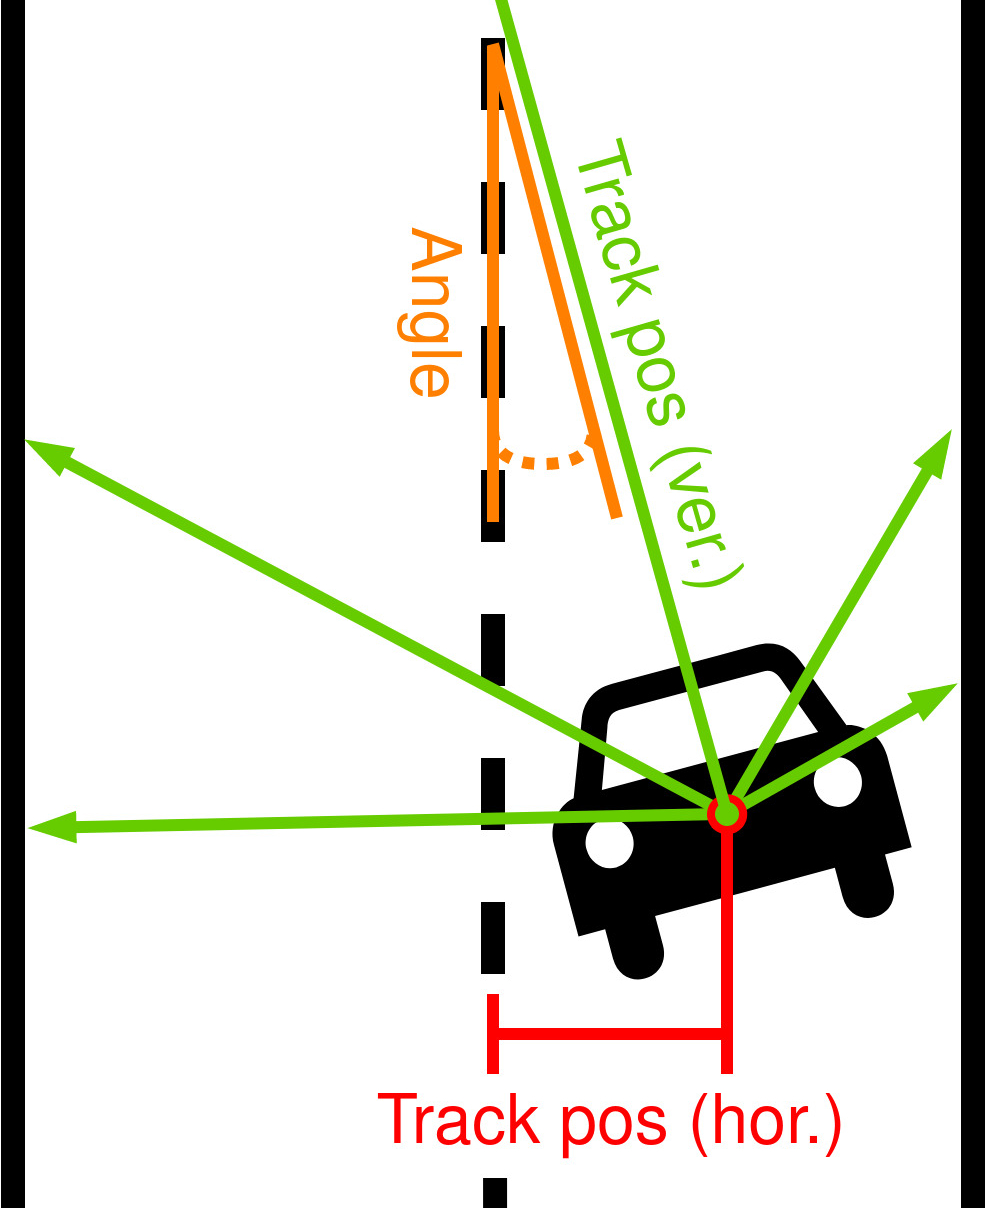
\includegraphics[width=0.3\linewidth]{figures/Observations.jpg}
    \centering
    \caption{Main environment observations}
    \label{fig:observations}
\end{figure}


\begin{tabularx}{\textwidth}{@{}p{0.18\textwidth}>{\centering}p{0.22\textwidth}X@{}}
\toprule
\textbf{Name}           & \textbf{Measurement}          & \textbf{Description}   \\ \midrule

\multicolumn{3}{@{}>{\centering}p{\linewidth}@{}}{\textit{Constant state parameters are not observed as they do not influence learning.} \textbf{The observations are not noisy.}} \\ \midrule

Angle          & [$-\pi$, $+\pi$] (rad) & Angle between car direction and track axis direction  \\ \midrule

Side force & ($-\inf$, $+\inf$) (km/h) & Speed along the transverse axis of the car. This is directly influenced by the steering actions of both human driver and agent. \\ \midrule

Track position (horizontal) & ($-\inf$, $+\inf$)     & Horizontal distance between the car and the track axis. $0$ when the car is on the axis, $+1$ if the car is on the left edge of the track, and $-1$ if the car is on the right edge of the track. Greater numbers than $+1$ or smaller numbers than $-1$ indicate that the car is off-track.  \\ \midrule

Track position (vertical)  & [$0$,$200$] (m) & Vector of 5 range finder sensors (of 19 available in TORCS). The range finders serve as lookahead by returning the distance between the car and the track edge in a given forward angle between $-90$ and $+90$ degrees with respect to the car axis. \\ \midrule 

Driver steering (last time step) & [$-1$, $+1$]  & The agent perceives the last input of the human. This is not the action of the human in the next but in the last time step. The agent does not know which action the human is going to choose simultaneous to its own action. $-1$ means full right (159 degrees) and $+1$ means full left (21 degrees).  \\ \bottomrule
\end{tabularx}

\subsection{Driver model}
\label{sec:driver_model}

The driver model is simplistic. If the driver is attentive, its actions are optimal. The driver model returns the action that steers the car as close to the center of the lane as possible. In this case, the agent should not interfere. However, if a distracted driver is modeled, the driver just repeats the last action it performed while being attentive. This can have the effect of the driver's action to overshoot with the car diverging from the center of the lane. Following, the agent has to identify distracted driving and counteract.

When the driver model is initialized, it is randomly set to be attentive or distracted. The driver stays in this state for a randomly chosen discrete time period between ten and 60 seconds for an attentive state and between two and six seconds for a distracted state. After the chosen time period, the state of attentiveness switches; a previously attentive driver becomes distracted, and a previously distracted driver becomes attentive. The process repeats until the experiment is over.

\subsubsection{Simple driver model}


\subsubsection{Steering over-correction}


\subsubsection{Steering over-correction and noise}

\subsection{Reward}

The overall goal for the agent is to only assist the driver in keeping the car centered in its lane. Therefore, this is the main source of reward for the agent. The more centered the car is at a certain time step, the more reward $r$ is received. However, the agent is supposed to leave the human driver with as much autonomy as possible. Thus, any intervention by the agent is penalized. Minor smooth interventions are generally preferred over large abrupt steering actions. Accordingly, the penalty is (exponentially) dependent on the intensity of the agent's action. The general assumption is that an attentive driver performs better in keeping the car centered than an inattentive driver. The agent has to predict whether a driver is attentive or not in order to choose its actions correctly. An incorrect prediction of the driver's actions will lead to overshooting and thus be negatively reflected in the reward for keeping the car centered. Lastly, the car is never supposed to leave the lane. Consequently, leaving the lane is highly penalized.


%For this reason, the penalty intensity is linked to the current distance of the car to the lane center; the higher the distance, the lower the agent's intervention penalty. On the other hand, 

% TODO: Add smoothing?

% \begin{equation}
%     \mathcal{R} = \mathcal{R}_{\textrm{center}} - \mathcal{P}_{\textrm{act position}} - \mathcal{P}_{\textrm{act intensity}} - \mathcal{P}_{\textrm{off-lane}}
% \end{equation}
\begin{equation*}
    \mathcal{R} = \mathcal{R}_{\textrm{center}} - \mathcal{P}_{\textrm{act intensity}} - \mathcal{P}_{\textrm{off-lane}}
\end{equation*}
\begin{equation*}
    \mathcal{R}_{\textrm{center}} = 
    \begin{cases}
        r - r * |Pos_{hor}| & \text{if} \quad |Pos_{hor}| \leq 1 \\
        0 & \text{if} \quad \text{off-lane}
    \end{cases}
\end{equation*}
% \begin{equation}
%     \mathcal{P}_{\textrm{act position}} = 
%     \begin{cases}
%         p_{\textrm{pos}} - p_{\textrm{pos}} * |Pos_{hor}| & \text{if} \quad |Pos_{hor}| \leq 1 \text{ and } \mathcal{A}_{\textrm{steer}}^{\textrm{agent}} \neq 0 \\
%         0 & \text{if} \quad \text{off-lane or no steering action}
%     \end{cases}
% \end{equation}
\begin{equation*}
    \mathcal{P}_{\textrm{act intensity}} = |\mathcal{A}_{\textrm{steer}}| ^ {p_{\textrm{int}}}
\end{equation*}
\begin{equation*}
    \mathcal{P}_{\textrm{off-lane}} = 
    \begin{cases}
        p_{\textrm{off}} & \text{if} \quad |Pos_{hor}| > 1 \\
        0 & \text{if} \quad |Pos_{hor}| \leq 1
    \end{cases}
\end{equation*}

\section{Solution approach using the POMCP algorithm}
\subsection{Discretization}
\label{sec:discretization}

\subsection{General POMCP definition}
\label{sec:pomcp}

% explain: 
% - Planning versus learning
% - How POMCP breaks the curse of dimensionality with Monte-Carlo sampling
% - Belief and blief update

% Particle filter belief update:
% See (POMDP, Thesis) Tactical Decision-Making forHighway Driving

% TODO: Replace planning time with number of searches
% TODO: Add select random
% TODO: Fix arrow for h = hao, s=s' (Use two diagonal arrows)
% TODO: Add caption
% TODO: Mark rollout and search phase as in the original paper
\begin{figure}[htbp]
    \centerfloat
    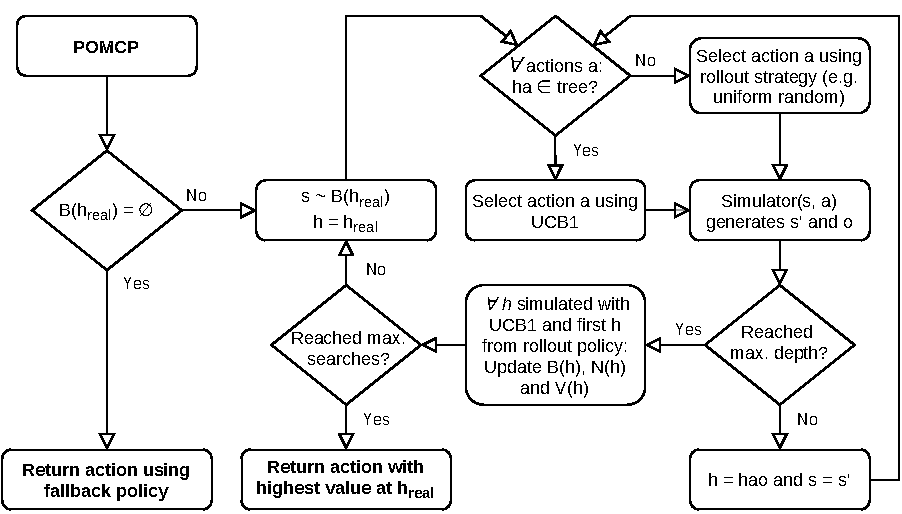
\includegraphics[width=1.2\textwidth]{figures/POMCP.pdf}
\end{figure}

\Gls{pomcp} constructs a search tree with nodes representing histories $h$ of actions and observations. At each node, $N(h)$ stores the number of times the represented history $h$ has been encountered, $V(h)$ is the node's value that is approximated by the average return of simulations starting at history $h$, and $B(h)$ represents the node's belief over the real environment's state. $B(h)$ is a collection of potential states where the likelihood of each state is given by the relative number of times it is included in the collection.

If the belief at the node representing $h_{real}$ is empty, an initial state distribution $I$ is used to sample a start state $s$ for the search. Otherwise, $B(h_{real})$ is utilized. The search tree is then searched in two stages. First, in the case that the search tree already contains child nodes for all actions at the current history, UCB1 is used for the action selection. Exploration is achieved by increasing the value of rarely-tried actions by an exploration bonus. Second, when the tree is missing a node for a potential action at the current history, a rollout policy is used to select actions. In the most simple case, this means choosing uniformly random over the action space. In either case, the selected action is executed on the start state $s$, leading to a successive state $s'$, observation $o$, and reward $r$. The process is repeated with resulting successive states until a maximum depth of the tree is reached. Afterwards, the beliefs, counts, and values are updated at all nodes for the histories resulting from the UCB1 action selection, and the node for the first history resulting from the rollout policy. The belief is updated by adding the successive states $s'$ from the simulator to the collections $B(ho)$ in the nodes. If the maximum planning time has not yet been reached, another start state is sampled and the whole process repeats. When the time runs out, the action $a_{best}$ with the highest value at the current history $h_{real}$ is returned. After this action is executed in the real environment, with an observation $o_{last}$ the tree can be pruned. Only the nodes from history $h_{real}a_{best}o_{last}$ onward stay relevant as all other histories are rendered impossible.

% TODO: Add particles as a construct (Or change particles everywhere else to "state in the belief")
% See Algorithms for decision making book

% One common approach is to use a particle filter, which represents the belief state as a collection of states. 10 Each state in the approximate belief is called a particle.

\subsection{Particle deprivation and particle injection}
\label{sec:particle_deprivation}

Particle filter approaches, POMCP included, can fail due to a phenomenon called particle deprivation. Because of the random nature of the process, the belief can sometimes converge towards a state that is far from the environment's true state. Particles that differ from the converged state have a low probability to be selected while sampling (low relative count). Hence, with each iteration, they become scarcer until they are completely erased from the belief. At this point, the agent is sure to be in an erroreous state and cannot recover anymore. Particle injection (also called particle reinvigoration) is a method to counteract this problem by introducing a number of random particles to the belief at each iteration \parencite{decision_making_book}. While this reduces the accuracy of the belief, it prevents its complete convergence towards a wrong state. 

Particle injection is used to increase the variance of the belief about the driver model state. Only observable information is used. Concretely, particle injection is implemented by adding driver model states with a random number of remaining actions and the same action as the one that was last observed. The number of remaining actions can be lower than the minimum defined in Section~\ref{sec:driver_model} because this limit is only intended for initial sampling and the true remaining number of driver actions in a particular state might be lower after having performed actions already. Like in the original POMCP paper, the amount of transformed particles that are added before each planning step is $1/16$ of the number of searches. The particles can be added during policy execution, and therefore, do not influence planning time.

% Use term posterior probability distribution? We can only add particles after making an observation so that we can verify that the potential particles to add match this belief.


\subsection{Action selection and preferred actions}
\label{sec:action_selection}

% TODO: Just say the agent does not act anymore when losing track with the belief instead of using uniformly random action selection? Makes more sense.

% This is strongly related to the particle deprivation problem described in Section~\ref{sec:particle_deprivation}. When the driver is in a distracted or attentive state, any number of remaining actions in this state below the maximum number (see Section~\ref{sec:driver_model}) could be valid and can therefore be part of the driver model states in the belief. In successive iterations, particles that represent drivers switching their state earlier than the true driver, and therefore change their steering behavior, are ruled out and removed from the belief. Thereby, after some iterations, driver model states that have the same or more remaining actions than the true state dominate the belief.

% preferred actions = domain knowledge


    \chapter*{Algorithm}
\label{sec:algorithm}

% TODO: Look at PSRs

% The bane of generative model approaches is that they are often strongly dependent on a good model of the system’s dynamics. Most uses of partially observable Markov decision processes (POMDPs), for example, assume a perfect dynamics model and attempt only to estimate state.

% behavior distributions of human drivers are unknown

\begin{itemize}
    \item Planning: Computational process that takes a model as input and produces or improves a policy for interacting with the modeled environment.
    \item Learning: Whereas planning methods use simulated experience generated by a model, learning methods use real experience generated by the environment.
\end{itemize}

\section{Model-based planning}

\subsection{Offline}

Only suitable for small to medium POMDP problems but very difficult to scale up to large problems as the number of future sceanarios that has to be considered grows exponentially with the size of the POMDP \parencite{despot}. Therefore, offline planning is not considered in this thesis. 

\subsection{Online}

\textbf{With black-box simulator:}
\begin{itemize}
    \item POMCP (Monte-Carlo tree search from the current belief using samples from a black-box simulator.)
    \item DESPOT (Avoids POMCP’s extremely poor worst-case behavior by evaluating policies on a small number of sampled scenarios.)
    \item DESPOT-IS (Importance sampling improves DESPOT’s performance when there are critical, but rare events, which are difficult to sample.)
    \item HyP-DESPOT (Parallelization speeds up online planning by up to several hundred times, compared with the original DESPOT algorithm.)
\end{itemize}

\subsection{Notes}

\begin{itemize}
    \item The black-box simulator might not be time-efficient enough to plan ahead sufficiently.
    \item Even if we would achieve an optimal policy for our simulation environment, the performance is bound by the accuracy of the ACT-R model in the human experiment. An improvement of the model is not possible as it is stationary.
\end{itemize}

\section{Model-free learning}

\begin{itemize}
    \item QMDP-Net (A QMDP-Net is an RNN that imposes structure priors for sequential decision making under partial observability. It embeds a Bayesian filter and the QMDP algorithm in the network. The hidden state of the RNN encodes the belief for POMDP planning.)
    \item BA-POMCP (Bayes-Adaptive Partially Observable Markov Decision Processes (BA-POMDPs) extend POMDPs to allow the model to be learned during execution. BA-POMCP extends the Monte-Carlo tree search method POMCP to BA-POMDPs.)
    \item FBA-POMCP (Monte-Carlo tree search method for F-POMDPs where the state if factored into multiple components. Only applicable to some specific domains where this factorization is possible.)
    \item \emph{PSR-MCTS} (Planning from scratch with model uncertainty, where an offline \emph{PSR model} were firstly learned and then combined with online Monte-Carlo tree search.)
\end{itemize}

\subsection{Notes}

\begin{itemize}
    \item Success in model-free reinforcement learning for POMDPs is pretty much limited to small-scale problems at this point.
    \item BA-POMDP: While the approaches listed above show promising performance on some problems the performance is very dependent on prior domain knowledge \parencite{ba-pomdp-online-offline}.
\end{itemize}

\section{POMCP}
    \chapter*{POMCP}
\setcounter{page}{1}
\label{sec:pomcp}

% explain: 
% - Planning versus learning
% - Curse of dimensionality and how POMCP breaks it with Monte-Carlo sampling
% - Define state space dimensinality of Torcs problem
% - Belief and blief update
% - unweighted particle filter
% Stages of the simulation

\section*{Algorithm}

\begin{figure}[h]
    \centering
    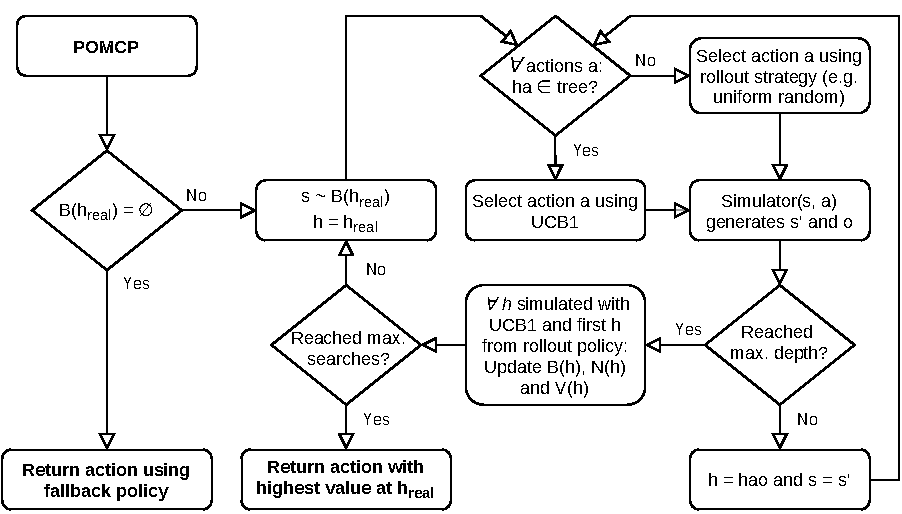
\includegraphics[width=\textwidth]{figures/POMCP.pdf}
\end{figure}

\Gls{pomcp} constructs a search tree with nodes representing histories $h$ of actions and observations. At each node, $N(h)$ stores the number of times the represented history $h$ has been encountered, $V(h)$ is the node's value that is approximated by the average return of simulations starting at history $h$, and $B(h)$ represents the node's belief over the real environment's state. $B(h)$ is a collection of potential states where the likelihood of each state is given by the relative number of times it is included in the collection.

If the belief at the node representing $h_{real}$ is empty, an initial state distribution $I$ is used to sample a start state $s$ for the search. Otherwise, $B(h_{real})$ is utilized. The search tree is then searched in two stages. First, in the case that the search tree already contains child nodes for all actions at the current history, UCB1 is used for the action selection. Exploration is achieved by increasing the value of rarely-tried actions by an exploration bonus. Second, when the tree is missing a node for a potential action at the current history, a rollout policy is used to select actions. In the most simple case, this means choosing uniformly random over the action space. In either case, the selected action is executed on the start state $s$, leading to a successive state $s'$, observation $o$, and reward $r$. The process is repeated with resulting successive states until a maximum depth of the tree is reached. Afterwards, the beliefs, counts, and values are updated at all nodes for the histories resulting from the UCB1 action selection, and the node for the first history resulting from the rollout policy. The belief is updated by adding the successive states $s'$ from the simulator to the collections $B(ho)$ in the nodes. If the maximum planning time has not yet been reached, another start state is sampled and the whole process repeats. When the time runs out, the action $a_{best}$ with the highest value at the current history $h_{real}$ is returned. After this action is executed in the real environment, with an observation $o_{last}$ the tree can be pruned. Only the nodes from history $h_{real}a_{best}o_{last}$ onward stay relevant as all other histories are rendered impossible.

    \chapter{Literature}
\label{sec:literature}

\iffalse

% FEEDBACK
% TODO: ACT-R Sources and better explanation
% TODO: Explain link between cogmod and rl agent


Model-based or model-free?

TODO: ADD HMM
Advantages of \gls{pomdp} over HMM:
Instead of single predicted state, a probability distribution over the possible states is considered
Allows the agent to actively take an action with the goal of reducing uncertainty about the human's state.

The scenario of a car with a human driver that is assisted by a \gls{rl} agent acting as \gls{adas} can be described as a \gls{pomdp}. From the perspective of the agent, the human is part of its environment. The agent can observe the car's sensory information and can perceive the human's actions. However, the agent is not aware if the human driver is attentive. Based on its observations, the agent must derive a probability distribution over the driver's level of attention (belief). Utilizing this, it tries to maximize its reward.

The \gls{pomdp} framework for \gls{hitl} control systems proposed by \cite{hitl_pomdp} serves as a foundation for this thesis. The driving task is extended from pure lane keeping, in a single lane without other road users, to multiple lanes with potential human-decided lane-switches, and other traffic participants with whom collisions have to be avoided. Moreover, continuous state and action spaces are considered.

\fi                                                                                                                                                                                                                                                                                 

% TODO reorder

This thesis focuses on efficient online \gls{pomdp} planning. The two most notable fast online \gls{pomdp} algorithms are DESPOT \parencite{despot} and POMCP \parencite{pomcp}. Both apply Monte Carlo tree search to evaluate the quality of candidate policies. At each time point, a simulator of the environment is used to form a search tree from multiple simulations in order to evaluate the resulting hypothetical histories by their mean return, leading to a real action of the agent in the environment and thus to a new real observation \parencite{pomcp}. DESPOT addresses and improves upon POMCP's problem of a poor worst-case performance bound \parencite{despot}.

Both POMCP and DESPOT can handle continuous state spaces but would have to be modified in order to support continuous action or observation spaces \parencite{online_pomdp_cont}. \citeauthor{online_pomdp_cont} provide two online algorithms for \gls{pomdp} with continuous state, action, and observation spaces: POMCPOW for simulating approximate state trajectories, and PFT-DPW for simulating approximate belief trajectories.

Offline and online approaches can be combined by using an approximate policy computed offline as a default policy \parencite{comb_online_offline}, or by considering a sequence of macro-actions to reduce the size of the search horizon \parencite{macro_actions}. Especially when there is only very little time for online planning, incorporating an offline approximation into an online approach can be useful \parencite{online_pomdp}.

\cite{hitl_pomdp} provide a framework for using a \gls{pomdp} to model a \gls{hitl} control system. Their framework serves as foundation for this thesis and is further described in \cref{sec:problem}. The framework is used in a case study where an agent assists a potentially drowsy human driver in keeping the car centered in its lane. Whether or not the driver is drowsy remains unknown to the agent. The agent's estimation of the driver's drowsiness is based on the humans actions such as turning the steering wheel and opening or closing its eyes. Intervention by the agent is possible both by alerting the driver with a warning, and by actively steering the car. Any intervention is penalized with the aim to interfere with the driver as little as possible but as much as required in order to keep the car centered when the driver is drowsy. They approximately solve their \gls{pomdp} problem with an offline randomized point-based value iteration approach. The policy is computed by iteratively sampling a finite set of random points from the agent's belief space. The agent thus interacts randomly with the environment in order to find an approximation of the optimal policy. The employed model of the human's internal state is rather simplistic and based on handcrafted transition probabilities. The state and action spaces are discrete.

\cite{att_intersec} evaluate how active probing can be utilized by autonomous vehicles in driving scenarios to reduce their uncertainty about a hidden psychological state of human drivers on the road. Three different scenarios are modeled: First, the agent wants to cross an intersections with other cars driving on the crossed road. The autonomous car can cautiously approach in order to probe the other cars for attentiveness; if they react by reducing their speed, they are likely attentive. Second, the agent drives on a highway with human drivers approaching from behind. The goal is to avoid rear-end collisions, which are especially likely in the case of inattentive human drivers. Active probing can be performed by the agent through braking. If an approaching driver does not slow down, the driver is most likely not paying attention. Third, the agent actively probes for an aggressive or timid driving style of other drivers by nudging into their lane. A human driver is expected to either slow down to allow the agent to switch lanes (timid driving style), or speed up to discourage the agent to switch lanes (agressive). This approach of actively provoking human responses rather than just passively observing leads to a significant improvement in classifying the human drivers' hidden attentiveness. It can potentially also be utilized in a shared control setting. The agent could utilize minor interventions to reduce uncertainty about the human's internal state.

Furthermore, the work of \cite{att_intersec} is relevant with regard to how they represent their problem as a \gls{pomdp} with a continuous state and action space and plan online using \gls{mpc}. At every time step, the agent uses an embedded human model to make predictions over a finite horizon about the actions a human would take in response to its own actions. The agent knows how a human would act in different psychological states, the state itself, however, is hidden. It is assumed that the human always tries to maximize its reward. The agent chooses a policy that maximizes its reward while accounting for the human's (potential) actions depending on the hidden psychological state the agent believes the human to be in. The real human actions that are observed after the agent executes an action are used to update the agent's belief about the human's internal state. The human model is learned a priori using \gls{irl} using demonstrations of human behavior for which the human's internal state is known.


% Shared control

\cite{shared_control} provide an overview of papers regarding decision making and human driver modeling for driver-vehicle shared control scenarios. Insight about recent developments, different architectures, and remaining challenges is provided. Of particular relevance are the different modes for the communication of authority between human and agent and the cognitive modeling approaches that are discussed.

% TODO: give examples of architectures





    \chapter{Experimental setup}
\label{sec:setup}

% TODO: Define terminal state

% TODO: Refine
The task for the agent in the experiment is to keep the car centered in a highway lane. Thus, the track used for the agent's evaluation needs to represent such a scenario. Most tracks readily available in the racing car simulator TORCS are race tracks. These are much wider than common roads and the width often differs in different segments. To ensure a realistic scenario, a one-lane track with a continuous width of 3.5m, which is common for European roads, is used. The track covers a wide array of scenarios. It includes long straight segments, both left and right curves, and multiple curves of alternating directions in a row. By ensuring that all common highway scenarios are covered by the track, a single track is sufficient.

The car used for the experiment does not have a big impact on driving performance, as long as it is consistent during all experiments. To ensure that an action's effect at a particular position are consistent, the speed of the car is constant.

The driver is pulled for an action every 0.1 seconds. The simulation tick rate is 0.002 seconds. When the driver is not pulled, its last action is repeated. It follows, that every action is repeated during 50 simulation ticks. The simulation is not in real time. Therefore, the simulation waits for the agent's planning. If the agent is pulled for an action, the environment does not change until the agent's next action is decided and performed.

\section{Evaluated scenarios}
\subsection{Driver model}
\subsection{Action space and action selection}
\section{Design decisions}
% TODO Leave out? Or add something useful here

\section{Hyperparameter optimization}

% TODO: Add parameter and hyperparameter table

% TODO: Refine
There are a number of hyperparameters. Most importantly, there is the planning time. This is the time the agent is allowed to search in and expand its search tree in order to find the most likely current state and best course of action. More planning time can result in a wider and/or deeper tree. The search horizon is limited by a discount threshold. If this threshold is reached, the search is stopped and no more actions will be performed for the current trajectory and, if there is enough planning time left, a new state is sampled from the current belief and a new planning trajectory is expanded. Moreover, there is an exploration constant. This value, determined before the start of the experiment, assigns actions that have not been tried before more expected reward and thus favors exploration.
\subsubsection{Number of searches}
\subsubsection{Exploration constant}
\subsubsection{Discount horizon}

\section{Performance metrics}
Due to the randomness involved in the driver model, each experiment run will lead to a different scenario. Therefore, to get credible results, the experiment has to be repeated many times. The average discounted return over all experiment runs serves as performance metric. This result is compared with the average reward of an agent that always performs the optimal reaction to the action of the driver model. The closer the POMCP agent's reward is to the optimal agent's reward, the better was the planning.


    \chapter{Research plan}
\label{sec:plan}

Writing a thesis is an iterative process. An overview of important goals, milestones, and deadlines is provided below and needs to be continually kept updated and revised. Weekly meetings are planned every Friday. To allow for a productive discussion, all milestones are due before these meetings. All dates are current estimates, some are purposefully left out to be set later.

%\begin{table}[hbtp]
\begingroup
    \centering
    \setlength\LTleft{0pt}
    \setlength\LTright{0pt}
    \begin{longtable}{l @{\extracolsep{\fill}} c}
        \toprule
        \textbf{Goal} & \textbf{Target date} \\ \midrule
        
        \textit{\textbf{Part 1: Theoretical setup}} &  \\ 
        Thesis outline    & 11-02-2021           \\\hdashline[1pt/10pt]
        Formulation of experiment design    & 11-02-2021 \\\hdashline[1pt/10pt]
        Performance evaluation criteria & 18-02-2021        \\\hdashline[1pt/10pt]
        Environment specification    & 18-02-2021           \\\hdashline[1pt/10pt] 
         
         & \\
        \textit{\textbf{Part 2: Agent design}} &  \\ 
        Contrasting potential algorithms (Pro/Con)    & 25-02-2021  \\\hdashline[1pt/10pt] 
        RL Algorithm decision    & 25-02-2021           \\\hdashline[1pt/10pt] 
        Detailed design of reward function    & 04-03-2021           \\\hdashline[1pt/10pt]
        \textbf{Finish Agent specification}    & 11-03-2021           \\\hdashline[1pt/10pt]
        
         & \\
        \textit{\textbf{Part 2: Practical setup}} &  \\ 
        Environment implementation in \gls{torcs}    & 11-03-2021           \\\hdashline[1pt/10pt] 
        
         & \\
        \textit{\textbf{Part 3: Agent implementation}} &  \\ 
        Language and framework decision & 18-03-2021           \\\hdashline[1pt/10pt] 
        Initial setup & 18-03-2021           \\\hdashline[1pt/10pt] 
        \textbf{Finish agent implementation}    & set later           \\\hdashline[1pt/10pt] 
        
         & \\
        \textit{\textbf{Part 5: Agent evaluation}} &  \\ 
        Agent tuning & set later  \\ \hdashline[1pt/10pt] 
        \textbf{Finish agent evaluation} (CogMod independent)   & set later          \\\hdashline[1pt/10pt] 
        \textbf{Finish agent}    & 14-06-2021           \\\hdashline[1pt/10pt] 

         & \\
        \textit{\textbf{Part 5: Human experiment (bonus chapter, not required)}} &                          \\ 
        Execute human experiment    & set later                               \\\hdashline[1pt/10pt] 
        \textbf{Assessment human experiment results}    & set later           \\\hdashline[1pt/10pt] 
        
         & \\
        \textit{\textbf{Part 6: Thesis preparation}} &  \\ 
        \textbf{Start writing}    & 01-07-2021           \\\hdashline[1pt/10pt] 
        
         
         & \\
        \textit{\textbf{Part 6: Wrap up}} &  \\ 
        \textbf{First final draft full thesis}    & 01-08-2021           \\\hdashline[1pt/10pt]
        Incorporate feedback    & set later           \\\hdashline[1pt/10pt] 
        \textbf{Finished thesis}    & 14-08-2021           \\\hdashline[1pt/10pt] 
        \textbf{Thesis defense}    & set later           \\\bottomrule
    \end{longtable}
\endgroup

    % \appendix           % "Chapter" is renamed "Appendix"
    % \appendixpage       % Similar to \part*{Appendices}, but appears in TOC

    % \include{sections/appendixA}

    \backmatter         % Folios in Arabic numerals, unnumbered chapters.

    \printbibliography

\end{document}